\section{TRIỂN KHAI BACK-END}
\subsection{Tổng quan về Vercel - Dịch vụ điện toán phi máy chủ}
\hspace*{1cm}
Sau khi đã triển khai thành công dịch vụ cơ sở dữ liệu trên \textit{Aiven Cloud}. Bước tiếp theo trong quá trình triển khai hệ thống đó là ta cần triển khai ở phía \textit{back-end}. Việc triển khai \textit{back-end} được thực hiện song song với quá trình phát triển mã nguồn, được gọi là quá trình triển khai liên tục \textit{(Continuous Deployment - CD)}. Việc thực hiện triển khai liên tục là điều cần thiết trong hầu hết các dự án phần mềm. Trước hết việc triển khai liên tục cho phép đội ngũ phát triển ở phía \textit{front-end} có thể dễ dàng tích hợp \textit{API} vào trong ứng dụng \textit{front-end} mà không cần phải chạy ứng dụng \textit{back-end} ở phía \textit{local}. Việc tích hợp liên tục cho phép nhà phát triển \textit{back-end} nhanh chóng cung cấp \textit{API} cho các chức năng bên phía \textit{front-end}. Ngoài ra triển khai liên tục cũng cải thiện chất lượng phần mềm thông qua việc áp dụng các quy trình kiểm tra tự động liên tục. Bằng cách phát hiện sớm các lỗi trong quá trình phát triển, các lỗi này có thể được khắc phục ngay lập tức, giảm thiểu rủi ro và chi phí liên quan đến việc sửa lỗi trong giai đoạn sau của vòng đời phần mềm. Hơn nữa, việc triển khai liên tục giúp các nhóm phát triển phản ứng linh hoạt hơn với phản hồi của các bên liên quan bao gồm phía đội ngũ \textit{front-end} cũng như phía người dùng, để từ đó đội ngũ \textit{back-end} có thể nhanh chóng cập nhật các thay đổi và đưa các thay đổi đó lên ứng dụng một cách trơn tru nhất.\\
\hspace*{1cm}
Hiện nay, có rất nhiều đơn vị cung cấp dịch vụ đám mây để triển khai \textit{Web API}, bao gồm các dịch vụ miễn phí cũng như trả phí. Trong đó có các nền tảng dịch vụ đám mây quen thuộc được sử dụng phổ biến nhất là \textit{Google Cloud}, \textit{Microsoft Azure} và \textit{Amazon Web Services}. Các dịch vụ triển khai thường theo hai dạng chính đó là \textit{serverful} và \textit{serverless}. Serverful là một dạng triển khai đám mây trong đó nhà phát triển và tổ chức phải quản lý cơ sở hạ tầng máy chủ, điều này bao gồm thiết lập, cấu hình, và bảo trì máy chủ vật lý hoặc ảo. Trong khi đó ở hướng ngược lại, serverless là một cách triển khai trong đó nhà cung cấp dịch vụ đám mây tự động quản lý cơ sở hạ tầng máy chủ. Các nhà phát triển viết mã ứng dụng và triển khai nó mà không cần quan tâm đến việc thiết lập, quản lý hoặc bảo trì các máy chủ. Trong phạm vi dự án này, nhóm sẽ thực hiện triển khai \textit{back-end} theo hướng serverless. Điều này sẽ đem lại những lợi ích nhất định có thể kể đến là:
\begin{itemize}
    \item \textit{Không cần quản lý server:} Nhà cung cấp dịch vụ đám mây chịu trách nhiệm về cơ sở hạ tầng. Nhà phát triển chỉ cần tập trung vào viết mã.
    \item \textit{Có thể tự động mở rộng:} Ứng dụng có thể tự động mở rộng để đáp ứng nhu cầu tải, mà không cần cấu hình thêm máy chủ thủ công.
    \item \textit{Chi phí thanh toán dựa trên mức độ sử dụng}: Bạn chỉ phải trả tiền cho thời gian thực thi mã của mình, không phải cho thời gian mà máy chủ nhàn rỗi.
    \item \textit{Thời gian khởi động nhanh:} Vì cơ sở hạ tầng được quản lý động, thời gian khởi động ứng dụng thường rất nhanh.
\end{itemize}
\hspace*{1cm}
Ở đây nhóm sẽ sử dụng dịch vụ \textit{Vercel}, Vercel là một nền tảng đám mây được thiết kế để triển khai và lưu trữ các ứng dụng web và front-end một cách nhanh chóng và dễ dàng. Nó cung cấp dịch vụ triển khai liên tục tự động, cho phép nhà phát triển đẩy mã mới lên kho lưu trữ và \textit{Vercel} sẽ tự động triển khai nó lên môi trường sản phẩm. \textit{Vercel} được xây dựng dựa trên mạng lưới toàn cầu của \textit{Edge servers}, giúp mang lại hiệu suất cao và độ trễ thấp cho người dùng toàn cầu, các lợi ích mà \textit{vercel} đem lại có thể kể đến như:
\begin{itemize}
    \item \textit{Triển khai ứng dụng web:} \textit{Vercel} có thể triển khai các ứng dụng \textit{web} tĩnh, ứng dụng \textit{React}, ứng dụng \textit{Vue.js}, \textit{Svelte} và các ứng dụng \textit{Node.js}.
    \item \textit{Lưu trữ tệp tĩnh:} \textit{Vercel} có thể lưu trữ và phân phối các tệp tĩnh như hình ảnh, \textit{CSS} và \textit{JavaScript}.
    \item \textit{Mạng CDN toàn cầu:} \textit{Vercel} sử dụng mạng \textit{CDN} toàn cầu để phân phối nội dung ứng dụng của nhà phát triển đến người dùng trên toàn thế giới một cách nhanh chóng và hiệu quả.
    \item \textit{Tên miền tùy chỉnh:} Nhà phát triển có thể sử dụng tên miền tùy chỉnh cho ứng dụng \textit{Vercel} của mình.
    \item \textit{HTTPS:} \textit{Vercel} hỗ trợ \textit{HTTPS} cho tất cả các ứng dụng.
    \item \textit{Analytics:} \textit{Vercel} cung cấp \textit{analytics} tích hợp để theo dõi lưu lượng truy cập và hiệu suất ứng dụng.
\end{itemize}
\subsection{Thực hiện triển khai back-end trên Vercel}
\hspace*{1cm}
Bước đầu tiên, ta cần có tài khoản \textit{Vercel} và thực hiện liên kết tài khoản tới trình quản lý \textit{Git}, có thể là \textit{GitHub}, \textit{GitLab} hoặc \textit{BitBucket}, ngoài ra cũng có thể thực hiện liên kết với trình quản lý \textit{Git} của bên thứ ba. Sau đó ở thư mục chứa mã nguồn \textit{back-end}, ta cần tạo một file đặt tên là \textit{vercel.json} để thiết lập cấu hình trước khi triển khai trên \textit{Vercel}. Dưới đây là đoạn mã cấu hình trong dự án \textit{back-end} của nhóm:
\begin{lstlisting}[language=json,firstnumber=1]
{
    "version": 2,
    "builds": [
        {
            "src": "src/main.ts",
            "use": "@vercel/node"
        }
    ],
    "routes": [
        {
            "src": "/(.*)",
            "dest": "src/main.ts",
            "methods": ["GET", "POST", "PUT", "PATCH", "DELETE", "OPTIONS"],
            "headers": {
                "Access-Control-Allow-Origin": "*"
            }
        }
    ]
}
\end{lstlisting}
\hspace*{1cm}
Bước tiếp theo, vì ta sử dụng \textit{Prisma ORM} để làm việc với cơ sở dữ liệu, nên sẽ cần thiết lập câu lệnh sẽ được chạy khi \textit{Vercel} thực hiện \textit{build} dự án để sinh ra được \textit{prisma client} trên \textit{Vercel}. Ở đây ta cần đề cập đến cơ chế hoạt động của \textit{Prisma ORM}, sau khi đặc tả các bảng và quan hệ trong \textit{file schema.prisma}, ta cần chạy câu lệnh \textit{prisma push} để đồng bộ với cơ sở dữ liệu ở trên \textit{server}. Khi thực hiện câu lệnh \textit{prisma push}, \textit{Prisma} cũng đồng thời thực thi câu lệnh \textit{prisma generate} để sinh ra \textit{prisma client} nằm ở trong thư mục của dự án. \textit{Prisma client} có thể được hiểu là \textit{API} trung gian mà \textit{Prisma} cung cấp để phía \textit{back-end} có thể giao tiếp được với cơ sở dữ liệu. Do vậy khi triển khai dự án trên \textit{Vercel}, ta cũng cần phải thiết lập để câu lệnh \textit{prisma generate} có thể thực thi đồng thời với quá trình \textit{build} dự án. Để làm được điều này ta cần chỉnh sửa ở \textit{file package.json} trong mã nguồn như sau:
\begin{lstlisting}[language=json,firstnumber=1]
{
    //...
    "scripts": {
        "build": "npm run generate-prisma-client-on-build && nest build",
        //...
        "generate-prisma-client-on-build": "prisma generate --schema prisma/schema.prisma",
        "vercel-build": "npm run build"
    }
    //...
}
\end{lstlisting}
\hspace*{1cm}
Đến đây ta đã thực hiện chỉnh sửa xong mã nguồn để sẵn sàng triển khai trên \textit{Vercel}, bước tiếp theo khá quen thuộc đó là ta cần \textit{commit} và \textit{push} những thay đổi mà ta đã thực hiện ở phía trên lên trên \textit{GitHub}. Sau khi đã thực hiện xong, ta sẽ truy cập vào trang chủ của \textit{Vercel} và khởi tạo một dự án triển khai mới. Trước tiên ta cần chọn tên của \textit{GitHub repository} tương ứng với dự án cần triển khai, sau đó nhấn vào \textit{Import}, lúc này \textit{Vercel} sẽ hiển thị giao diện để thực hiện các cấu hình cần thiết trước khi triển khai dự án. Tại bước thiết lập này, ta sẽ cần đặt tên cho dự án triển khai ở mục \textit{Project Name}, chọn \textit{framework} ứng với dự án, vì ở đây ta triển khai dự án \textit{NestJS} nên không có tùy chọn tương ứng, do đó ở mục \textit{Framework Preset} ta sẽ chọn \textit{Other}. Tiếp theo ở mục \textit{Root Directory}, ta cần trỏ tới thư mục chứa toàn bộ mã nguồn của dự án, mặc định ta không cần thay đổi ở mục này, tuy nhiên với \textit{Git repository} mà có chứa nhiều dự án khác thì ta cần thiết lập cho chính xác. Tiếp theo cần thiết lập ở mục \textit{Build and Output Settings}, vì đây là dự án \textit{NestJS} nên ở mục này ta không cần tùy chỉnh, tuy nhiên cần lưu ý với các dự án khác nhau. Cuối cùng ta cần thêm các biến môi trường của dự án ở mục \textit{Environment Variables}, chúng ta có thể thêm một cách tiện lợi đó là \textit{copy} toàn bộ \textit{file .env} trong dự án và \textit{paste} vào ô đầu tiên của mục này, tất cả các biến môi trường sẽ tự động được \textit{import}.
\begin{figure}[H]
    \centering
    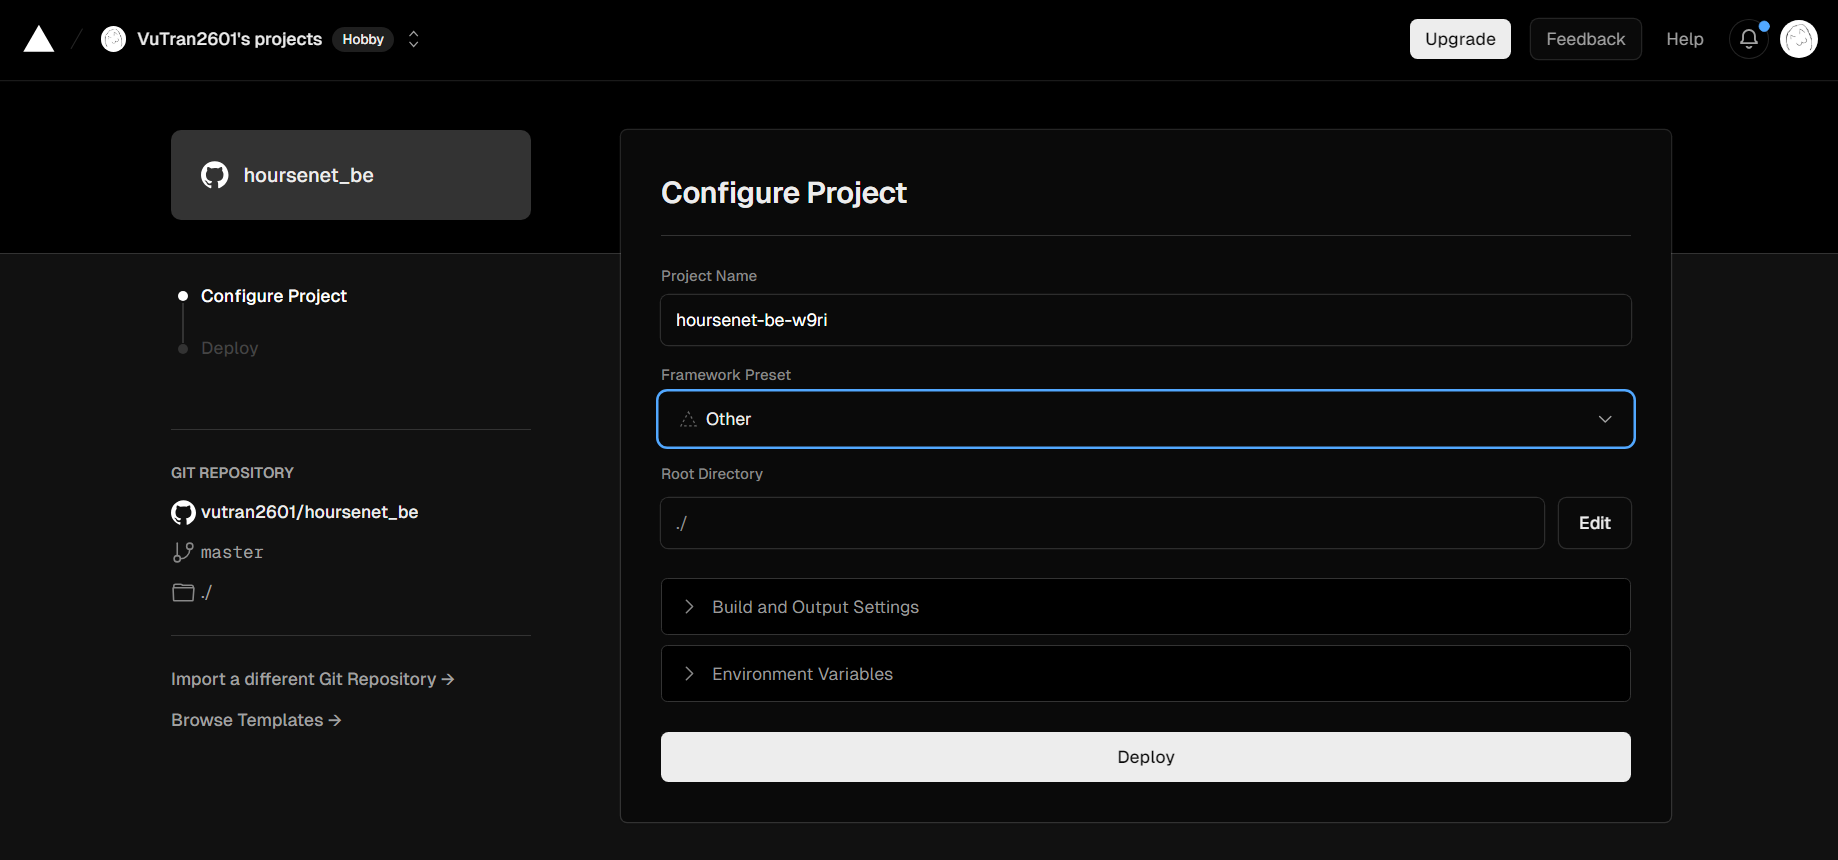
\includegraphics[width=1\textwidth]{Images/Deployment/Backend/VercelConfig.png}
    \caption{Thiết lập cấu hình trước khi triển khai dự án trên Vercel}
\end{figure}
\hspace*{1cm}
Sau khi đã hoàn tất các bước ở trên, ta sẽ nhấn vào \textit{Deploy} để \textit{Vercel} tiến hành triển khai ứng dụng, để theo dõi quá trình \textit{build}, ta có thể quan sát ở mục \textit{Deployment Details}, tại mục này sẽ hiển thị các tiến trình \textit{Vercel} thực hiện \textit{build} và triển khai ứng dụng, ta có thể nhấn vào chi tiết để xem các câu lệnh được chạy trong quá trình \textit{build}, nhờ đó ta có thể theo dõi quá trình \textit{build} có thành công hay không, hoặc nếu xảy ra lỗi, ta có thể xem \textit{build log} để tìm ra nguyên nhân gây ra lỗi khi \textit{build} ứng dụng.
\begin{figure}[H]
    \centering
    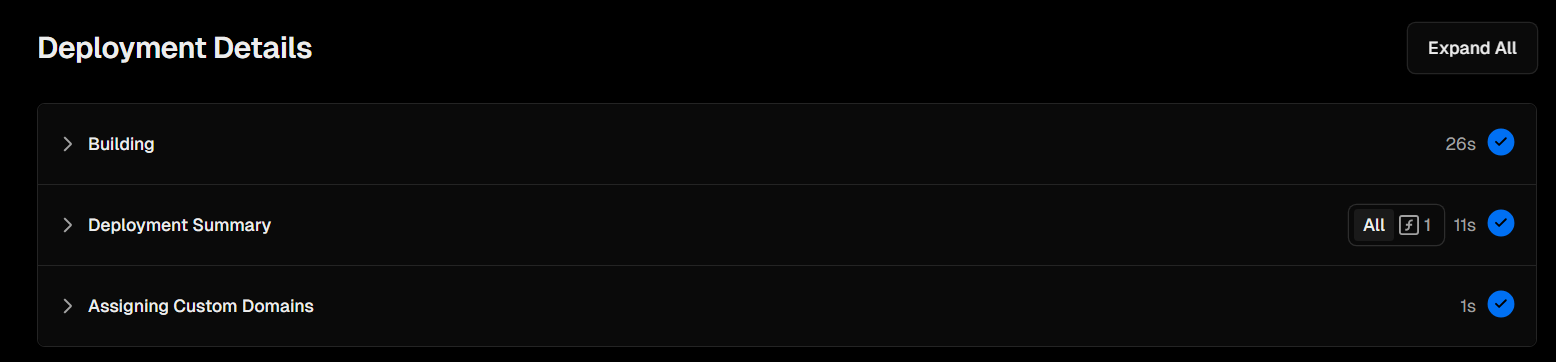
\includegraphics[width=1\textwidth]{Images/Deployment/Backend/DeploymentDetail.png}
    \caption{Các bước build ứng dụng trên Vercel}
\end{figure}
\begin{figure}[H]
    \centering
    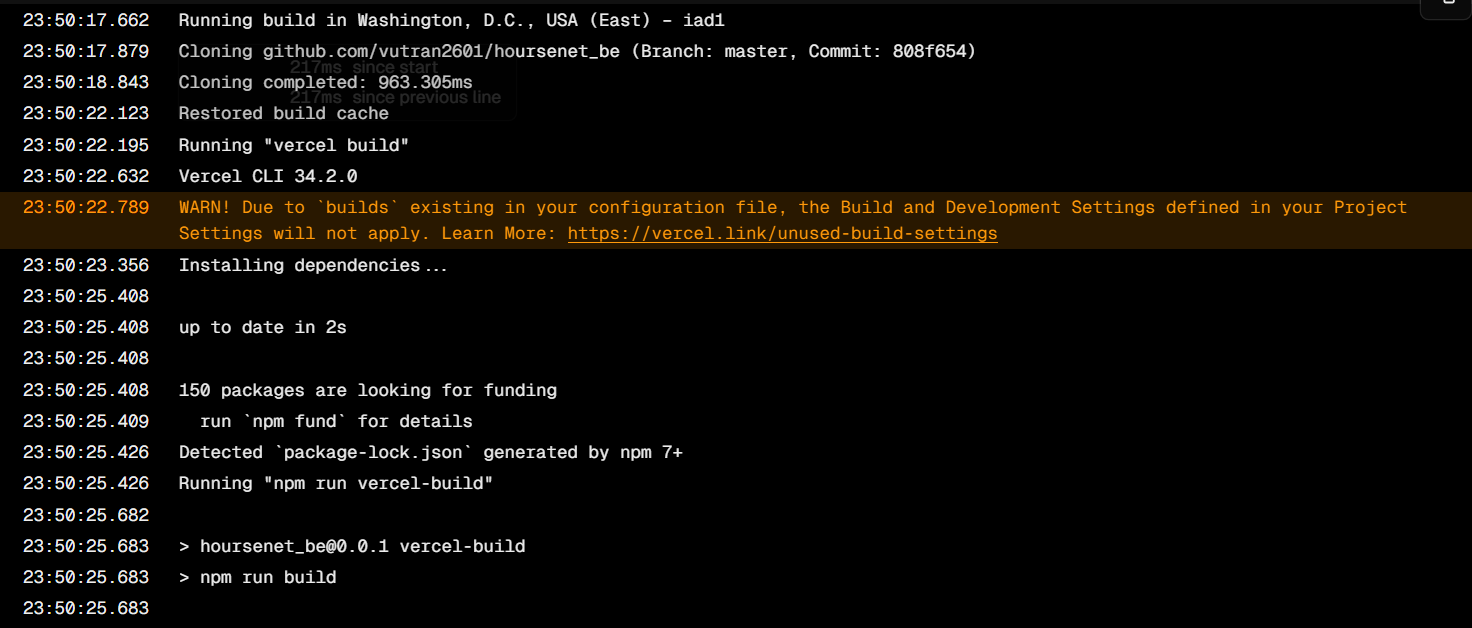
\includegraphics[width=1\textwidth]{Images/Deployment/Backend/BuildLog.png}
    \caption{Build log hiển thị các câu lệnh được thực thi khi Vercel build ứng dụng}
\end{figure}
\hspace*{1cm}
Khi khởi tạo dự án triển khai trên \textit{Vercel}, ở lần \textit{build} đầu tiên, \textit{Vercel} sẽ cung cấp một tên miền với cấu trúc là \url{[project-name].vercel.app}. Sau khi quá trình \textit{build} thành công và không gặp bất cứ lỗi nào, kết quả thành công sẽ được hiển thị trên giao diện chính của dự án, và ta có thể sử dụng tên miền mà \textit{Vercel} cung cấp để tích hợp ở phía \textit{front-end}. Ngoài ra ta cũng có thể truy cập vào \textit{tab Log} để theo dõi ứng dụng hoạt động.
\begin{figure}[H]
    \centering
    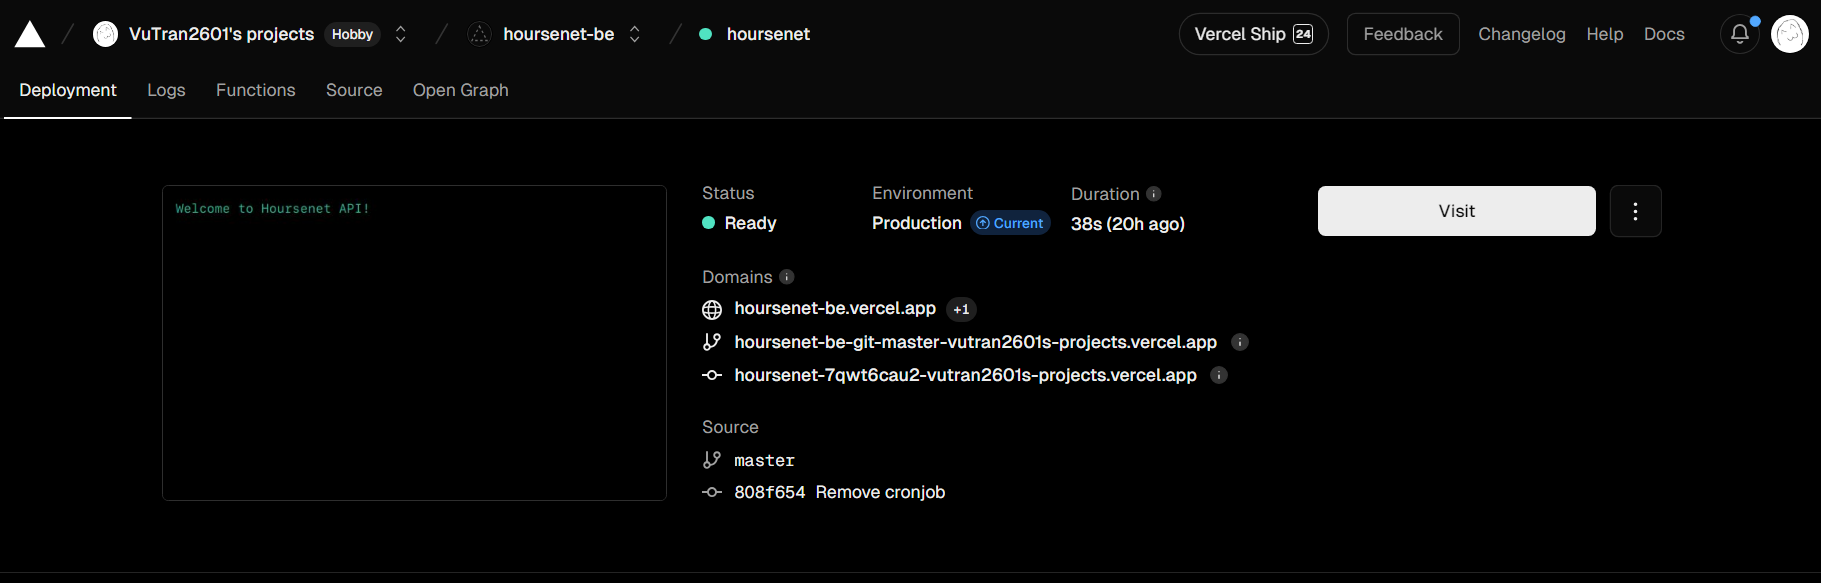
\includegraphics[width=1\textwidth]{Images/Deployment/Backend/SuccessfullyBuilt.png}
    \caption{Kết quả sau khi build ứng dụng thành công trên Vercel}
\end{figure}